\documentclass{article}
\usepackage[utf8]{inputenc}
\usepackage{fancyhdr}
\usepackage{polski}
\usepackage{mathtools}
\usepackage{ulem}
\usepackage[margin = 1cm]{geometry}
\usepackage{hhline}
\usepackage{array}
\usepackage{booktabs}
\usepackage{tabularx}
\usepackage{colortbl}
\usepackage{longtable}
\usepackage{mathdots}
\usepackage{multirow}
\usepackage{centernot}
\usepackage{tensor}
\usepackage{fancyhdr}
\usepackage{lastpage}
\usepackage{enumitem}
\usepackage{amsthm}
\usepackage{mathabx}
\usepackage{algpseudocode}
\usepackage{algorithm}
\usepackage{pgfplots}


\title{Sprawozdanie Obliczenia Naukowe}
\author{Piotr Zapała}
\date{November 2023}
\begin{document}
\maketitle

\tableofcontents
\newpage
\begin{center}
    \section{Zadanie 1}
    \subsection{Opis problemu}
    \large W zadaniu pierwszym jesteśmy proszeni o zaimplementowanie funkcji która oblicza ilorazy różnicowe.
    \texttt{function ilorazyRoznicowe(x::Vector{Float64}, f::Vector{Float64})} \newline
     Nasza funkcja powinna przyjmować jako argumenty następujące parametry: \newline
     \begin{flushleft}
        \textbf{Dane:} \newline  
        \textbf{x} - wektor długości \(n + 1\) zawierający węzły \(x_{0}, \dots ,x_{n}\),   \(x[1] = x_{0},\dots,x[n+1]=x_{n}\) \newline
        \textbf{f} - wektor długości \(n + 1\) zawierający wartości interpolowanej funkcji w węzłach \(f(x_{0}),\dots,f(x_{n})\).
     \end{flushleft}
     Zaimlementowana funkcja \texttt{"ilorazyRoznicowe"} powinna zwracać następujące wyniki: \newline
     \begin{flushleft}
        \textbf{Wyniki:} \newline  
        \textbf{fx} - wektor długości \(n + 1\) zawierający obliczone ilorazy różnicowe \newline
        \(fx[1] = f[x_{0}], fx[2] = f[x_{0},x_{1}],\dots,fx[n] = f[x_{0},\dots,x_{n-1}], fx[n+1] = f[x_{0},\dots,x_{n}]\).  
     \end{flushleft}
      Autor powyższego zadania wymaga aby nasza funkcja została zaimplementowana bez użycia tablicy dwuwymiarowej (macierzy).

    \subsection{Rozwiązanie}
    \large W celu obliczania ilorazów różnicowych wyższych rzędów, należy się posłużyć poniższym rekurencyjnym wzorem.
    \[f[x_{i},x_{i+1},\dots,x_{i+j}]=\frac{f[x_{i},x_{i+2},\dots,x_{i+j}]-f[x_{i},x_{i+1},\dots,x_{i+j-1}]}{x_{i+j}-x_{i}}\] \newline
    Jeśli znamy węzły \(x_{i}\) oraz wartości funkcji \(f(x_{i})\), czyli ilorazy zerowego rzędu, jesteśmy w stanie za pomocą powyższego wzoru utworzyć
    tablicę ilorazów różnicowych wyższych rzędów. \newline Przykładowa tablica ilorazów w przypadku, gdy znamy cztery węzły może wyglądać następująco: \newline
    \begin{flushleft}
    \(x_{0}\;f[x_{0}]\;|\;f[x_{0},x_{1}]\;f[x_{0},x_{1},x_{2}]\;f[x_{0},x_{1},x_{2},x_{3}]\) \newline
    \(x_{1}\;f[x_{1}]\;|\;f[x_{1},x_{2}]\;f[x_{1},x_{2},x_{3}]\) \newline
    \(x_{2}\;f[x_{2}]\;|\;f[x_{2},x_{3}]\) \newline
    \(x_{3}\;f[x_{3}]\;|\)
    \end{flushleft}
    Pionowa kreska oddziela wielkości dane od obliczonych. \newline
    Pierwszy wierz tablicy zawiera iloraz, które wystepują we wzorze interpolacyjnym Newtona. \newline

    Jeżeli przyjmiemy, że \(c_{ij}=f[x_{i},x_{i+1},\dots,x_{i+j}]\), nasza tablica ilorazów różnicowych ma następującą postać: \newline
    \begin{flushleft}
        \(x_{0}\;\;\;\;\;\;\;c_{00}\;\;\;|\;c_{01}\;\;\;\;\;c_{02}\;\;\;\;\;\dots\;\;\;\;\;c_{0,n-1}\;\;\;\;\;c_{0n}\) \newline
        \(x_{1}\;\;\;\;\;\;\;c_{10}\;\;\;|\;c_{11}\;\;\;\;\;c_{12}\;\;\;\;\;\dots\;\;\;\;\;c_{1,n-1}\) \newline
        \(\dots\;\;\;\;\;\;\dots\;\;|\;\dots\;\;\;\;\dots\) \newline
        \(x_{n-1}\;c_{n-1,0}\;|\;c_{n-1,1}\) \newline
        \(x_{n}\;\;\;\;\;\;c_{n0}\;\;\;|\)
    \end{flushleft}

    Nasz wzór rekurencyjny przyjmuje następującą postać: \newline
    \[c_{ij}=\frac{c_{i+1,j-1}-c_{i,j-1}}{x_{i+j}-x_{i}}\]

    Zgodnie z wymaganiami autora, algorytm obliczania ilorazów różnicowych powinien wykonywać obliczenia bez użycia tablicy dwuwymiarowej.
    Aby osiągnąć wymagany efekt należy użyć tablicy \(d\), początkową wartością zmiennej \(d_{i}\) jest \(c_{0}=f(x_{i})\) z drugiej kolumny trójkątnej tablicy ilorazów,
    następnymi wartościami - wielkości \(c_{i-1,1},\dots,c_{1,i-1},c_{0i}\). Aby tablica \(d\) zawierała w każdej chwili ilorazy, które będą potrzebne później,
    należy tworzyć naszą tablicę kolumnami, a w każdej kolumnie - z dołu do góry. \newline
    \begin{flushleft}
        \begin{algorithm}
            \caption{ilorazyRoznicowe}\label{alg:ilorazyRoznicowe}
            \begin{algorithmic}
                \Function{ilorazyRoznicowe}{$x, f$}
                \State$n \gets length(f)$
                \For {$i \leftarrow 0, n$}
                    \State$d[i] \gets f(x_{i})$
                \EndFor
                \For {$j \leftarrow 1, n$}
                    \For {$i \leftarrow n, j$}
                        \State$d_{i} \gets (d_{i}-d_{i-1})/(x_{i}-x_{i-j})$
                    \EndFor
                \EndFor \newline
                \Return{$d$}
                \EndFunction
            \end{algorithmic}
        \end{algorithm}
    \end{flushleft}
    \section{Zadanie 2}
    \subsection{Opis problemu}
     \large W zadaniu drugim należy napisać funkcję obliczającą wartość wielomianu interpolacyjnego stopnia \(n\) w postaci Newtona
      \(N_{n}(x)\) w punkcie \(x = t\) za pomocą uogólnionego algorytmu Hornera, w czasie \(O(n)\). \newline
      \texttt{function warNewton(x::Vector{Float64}, fx::Vector{Float64}, t::Float64)} \newline
       Nasza funkcja powinna przyjmować jako argumenty następujące parametry: \newline
      \begin{flushleft}
        \textbf{Dane:} \newline  
        \textbf{x} - wektor długości \(n + 1\) zawierający węzły \(x_{0}, \dots ,x_{n}\),   \(x[1] = x_{0},\dots,x[n+1]=x_{n}\) \newline
        \textbf{fx} - wektor długości \(n + 1\) zawierający obliczone ilorazy różnicowe \newline
        \(fx[1] = f[x_{0}], fx[2] = f[x_{0},x_{1}],\dots,fx[n] = f[x_{0},\dots,x_{n-1}], fx[n+1] = f[x_{0},\dots,x_{n}]\). \newline
        \textbf{t} - punkt, w którym należy obliczyc wartość wielomianu
     \end{flushleft}
     Zaimlementowana funkcja \texttt{"warNewton"} powinna zwracać następujący wynik: \newline
     \begin{flushleft}
        \textbf{Wyniki:} \newline  
        \textbf{nt} - wartość wielomianu w punkcie \(t\). 
     \end{flushleft}
 
    \subsection{Rozwiązanie}
    \large Rozwiązanie zadania polega na zaimplementowaniu uogólnionego algorytmu Hornera, w czasie \(O(n)\). \newline
     Schemat Hornera jest algorytmem służącym do bardzo szybkiego obliczania wartości wielomianu. \newline
     Mamy wielomian w postaci naturalnej \(p(x)=a_{0}x^n+a_{1}x^{n-1}+\cdots+a_{n}\), gdzie współczynniki \(a_{0},a_{1},\dots,a_{n}\)
     mogą być liczbami rzeczywistymi lub zespolonymi, natomiast \(x\) jest zmienną niezależną. \newline
     Naszym zadaniem jest znaleźć wartość \(p(c)=?\), w dowolnym punkcie rzeczywistym \(x=c\). \newline
     \newpage
     Ilość operacji jakie należy wykonać aby wyliczyć wartośc \(p(c)\) to: \newline
     \begin{flushleft}
        - \(n\) dodawań \newline
        - \(n\) mnożeń \((a_{0}*x^n,a_{1}*x^{n-1},\dots,a_{n-1}*x)\) \newline
        - \(n-1\) mnożeń \((x^2, x^3,\dots,x^n)\) \newline
     \end{flushleft}
     W sumie do obliczenia wartości wielomian \(p(x)\) w punkcie \(x=c\) potrzeba \(3n-1\) operacji. \newline

     Z pomocą algorytmu Hornera jesteśmy w stanie zmniejszyć ilość wykonywanych operacji. \newline 
     Po podzieleniu wielomianu \(p(x)=a_{0}x^n+a_{1}x^{n-1}+\cdots+a_{n}\) przez dwumian \(x-c\) otrzymujemy: \newline
     \(p(x)=(x-c)*q(x)+b_{n}\), gdzie \(q(x)=b_{0}x^{n-1}+b_{1}x^{n-2}+\cdots+b_{n-1}\), \newline oraz \(b_{n}\) jest resztą z dzielenia \(p(x)\) przez \(x-c\), \(b_{n}=p(c)\). \newline

     Z powyższych wzorów wynika, że \newline
     \[a_{0}x^n+a_{1}x^{n-1}+\cdots+a_{n}=(x-c)(b_{0}x^{n-1}+b_{1}x^{n-2}+\cdots+b_{n-1})+b_{n}=\]
     \[=b_{0}x^n+(-b_{0}*c+b_{1})x^{n-1}+(-b_{1}*c+b_{2})x^{n-2}+\cdots+(-b_{n-1}*c+b_{n})\] \newline
     Jeśli powrównamy współczynniki przy \(x^i, i = n,\ldots,0\), otrzymamy następujący algorytm: \newline
     \begin{flushleft}
        \(a_{0}=b_{0}\) \newline
        \(a_{1}=-b_{0}*c+b_{1}\) \newline
        \(a_{2}=-b_{1}*c+b_{2}\) \newline
        \(\vdots\) \newline
        \(a_{n}=-b_{n-1}*c+b_{n}\) \newline

        Stąd otrzymujemy: \newline

        \(b_{0}=a_{0}\) \newline
        \( b_{i}=b_{i-1}*c+a_{1},i=1,2,\ldots,n\) \newline 
        \(b_{n}=p(c)\)
     \end{flushleft}
     Koszt algorytmu to \(2n\) działań, mamy \(n\) mnożeń i \(n\) dodawań. \newline 

     Powyższy algorytm można bez jakichkolwiek problemów stosować do obliczenia wartości wielomianu w zadanym punkcie, natomiast 
     warto zwrócić uwagę, iż wielomian musi być w postaci naturalnej. W naszym zadaniu musimy obliczyć wartość wielomianu interpolacyjnego Newtona, który jest w następującej postaci: \newline
     \[p(x) = a_{0} + \sum_{i=1}^{n} a_{i} \prod_{j=0}^{i-1} (x-x_{j}) = a_{0} + a_{1}(x-x_{0}) + a_{2}(x-x_{1})(x-x_{0})+\cdots+a_{n}(x-x_{n-1})\cdots(x-x_{1})(x-x_{0})\] \newline
     Gdzie \(a_{0},a_{1},\ldots,a_{n}\), to ilorazy różnicowe, a \(x_{0},x_{1},\ldots,x_{n-1}\) węzły interpolacyjne. \newline
     Zatem powyższą zależność można przedstawić używając ogółnionych wzorów Hornera. \newline 
     \[w_{n}(x)=f[x_{0},\dots,x_{n}]\]
     \[w_{k}=f[x_{0},\dots,x_{k}]+(x-x_{k})*w_{k+1}(x), \;k\in[n-1,0]\] 
     \newpage
     Powyższe zależnośći możemy już w łatwy sposób przełożyć na kod, który prezentuje się następująco:
     \begin{flushleft}
        \begin{algorithm}
            \caption{warNewton}\label{alg:warNewton}
            \begin{algorithmic}
                \Function{warNewton}{$x, fx, t$}
                \State$n \gets length(fx)$
                \State$b \gets fx[n]$
                \For {$i \leftarrow n-1, 1$}
                    \State$b \gets fx[i] + (t - x[i]) * b$
                \EndFor \newline
                \Return{$b$}
                \EndFunction
            \end{algorithmic}
        \end{algorithm}
    \end{flushleft}
    \section{Zadanie 3}
    \subsection{Opis problemu}
    \large Zadanie trzecie polega na zaimplementowaniu funkcji obliczającej współczynniki wielomianu w postaci naturalnej 
     \(a_{0},\dots,a_{n}\) tzn. \(a_{n}x^{n} + a_{n-1}x^{n-1} + \dots + a_{1}x + a_{0}\).
     W celu obliczenia współczynników w postaci naturalnej należy posłużyć się współczynnikami wielomianu interpolacyjnego w postaci Newtona 
     \(c_{0} = f[x_{0}], c_{1} = f[x_{0}, x_{1}], c_{2} = f[x_{0},x_{1},x_{2}],\dots,c_{n} = f[x_{0},\dots,x_{n}]\) oraz węzłami \(x_{0},x_{1},\dots,x_{n}\). \newline
     Autor zadania wymaga aby nasza funkcja działała w czasie \(O(n^{2})\). \newline 
     \texttt{function naturalna(x::Vector{Float64}, fx::Vector{Float64})} \newline 
     Nasza funkcja powinna przyjmować jako argumenty następujące parametry: \newline
     \begin{flushleft}
        \textbf{Dane:} \newline  
        \textbf{x} - wektor długości \(n + 1\) zawierający węzły \(x_{0}, \dots ,x_{n}\),   \(x[1] = x_{0},\dots,x[n+1]=x_{n}\) \newline
        \textbf{fx} - wektor długości \(n + 1\) zawierający obliczone ilorazy różnicowe \newline
        \(fx[1] = f[x_{0}], fx[2] = f[x_{0},x_{1}],\dots,fx[n] = f[x_{0},\dots,x_{n-1}], fx[n+1] = f[x_{0},\dots,x_{n}]\). \newline
     \end{flushleft}
     Zaimplementowana funkcja \texttt{"naturalna"} powinna zwracać następujący wynik: \newline
     \begin{flushleft}
        \textbf{Wyniki:} \newline  
        \textbf{a} - wektor długości \(n + 1\) zawierający obliczone współczynniki postaci naturalnej \newline
        \(a[1]=a_{0}, a[2]=a_{1},\dots,a[n]=a_{n-1}, a[n+1]=a_{n}\).
     \end{flushleft}
    \subsection{Rozwiązanie}
    \large Jak się okazuję, jeżeli zaczniemy się cofać jak algorytmie Hornera, jesteśmy w stanie wyliczyć wartość przy obecnej potędze.
     Przykładowo dla \(x^i\) mamy \(c_{i}-x_{i}a_{i+1}\), następnie należy zaktualizować współczynniki przy wyższych potęgach naszego wielomianu.
     Można zauważyć, iż dla każdego \(a_{j}\) w i-tej iteracji, dodajemy \(-x_{n-1}a_{j+1}\).
    Powyższe rozważania prowadzą nas do zaprojektowania algorytmu wyliczającego współczynniki w postaci naturalnej.
    \begin{flushleft}
        \begin{algorithm}
            \caption{naturalna}\label{alg:naturalna}
            \begin{algorithmic}
                \Function{naturalna}{$x, f$}
                \State$n \gets length(x)$
                \For {$i \leftarrow 0, n$}
                    \State$a[i] \gets 0$
                \EndFor
                \State$a[n] \gets fx[n]$
                \For {$i \leftarrow (n-1), 1$}
                    \State$a[i] \gets fx[i] - x[i] * a[i+1]$
                    \For {$j \leftarrow (i+1), (n-1)$}
                        \State$a[j] \gets a[j] - x[i] + a[j+1]$
                    \EndFor
                \EndFor \newline
                \Return{$a$}
                \EndFunction
            \end{algorithmic}
        \end{algorithm}
    \end{flushleft}
    \newpage

    \section{Zadanie 4}
    \subsection{Opis problemu}
     \large W zadaniu czwartym jesteśmy proszeni aby zaimplementować funkcję, która zinterpoluje zadaną funkcję \(f(x)\)
     za pomocą wielomianu interpolacyjnego stopnia \(n\) w postaci Newtona. \newline
     Następnie narysuje wielomian interpolacyjny i interpolowaną funkcję. W celu narysowania wykresu naszej funkcji można się posłużyć następującymi pakietami \texttt{Plots, PyPlot lub Gadfly}. \newline 
     W interpolacji należy użyć węzłów równoległych, tj. \(x_{k} = a + kh, h = \frac{(b-a)}{n}, k = 0,1,\dots,n\). \newline
     Autor zadania wymaga, abyśmy nie wyznaczali wielomianu interpolacyjnego w postaci jawnej. \newline
     Powinniśmy skorzystać z funkcji \texttt{ilorazyRoznicowe} i \texttt{warNewton}. \newline
     \texttt{function rysujNnfx(f, a::Float64, b::Float64, n::Int)} \newline
     Nasza funkcja powinna przyjmować jako argumenty następujące parametry: \newline
     \begin{flushleft}
        \textbf{Dane:} \newline  
        \textbf{f} - funkcja \(f(x)\) zadana jako anonimowa funkcja \newline
        \textbf{a, b} - przedział interpolacji \newline
        \textbf{n} - stopień wielomianu interpolacyjnego
     \end{flushleft}
     Zaimlementowana funkcja \texttt{"rysujNnfx"} powinna zwracać następujący wynik: \newline
     \begin{flushleft}
        \textbf{Wyniki:} \newline  
        - zaimplementowana funkcja rysuje wielomian i interpolowaną funkcję w przedziale \([a,b]\)
     \end{flushleft}

    \subsection{Rozwiązanie}
    \large Celem zadania czwartego jest połączenie zaimplementowanych metod w program pozwalający na rysowanie wykresów funkcji podanych do interpolacji, 
     jak również rysowanie zinterpolowanej funkcji. Autor zadania zarzyczył sobie, aby nie wyznaczać wielomianu interpolacyjnego w jawnej postaci, stąd potrzeba użycia zaimplementowanych metod.
     Funkcja powinna wykonać interpolacje na podanym przedziale \([a,b]\), dodatkowo należy użyć węzłów równoległych, stąd \(x_{k} = a + kh, h = \frac{(b-a)}{n}, k = 0,1,\dots,n\). \newline
     Dzięki możliwości rysowania wykresów, osoba korzystająca z programu, \newline jest w stanie porównać reprezentację graficzną danego problemu. \newline
     \newpage 
                            Poniższy pseudokod obrazuję sposób wykonania zadania.
    \begin{flushleft}
    \begin{algorithm}
    \caption{rysujNnfx}\label{alg:rysujNnfx}
    \begin{algorithmic}
    \Function{rysujNnfx}{$f, a, b, n$}
    \State$h \gets \frac{(b-a)}{n}$
    \For {$j \leftarrow 0, n$}
        \State$x[j] \gets 0$
        \State$y[j] \gets 0$
    \EndFor
    \For {$k \leftarrow 0, n$}
        \State$x[k+1] \gets a +k*h$
        \State$y[k+1] \gets f(x[k+1])$
    \EndFor
    \State$x \gets ilorazyRoznicowe(x, y)$
    \State$points \gets 50*(n+1)$
    \State$dx \gets \frac{b-a}{points-1}$
    \For {$z \leftarrow 0, points$}
        \State$func[z] \gets 0$
        \State$xs[z] \gets 0$
        \State$polynomial[z] \gets 0$
    \EndFor
    \State$xs[1] \gets a$
    \State$polynomial[1] \gets func[1] \gets y[1]$
    \For {$i \leftarrow 2, points$}
        \State$xs[i] \gets xs[i-1] + dx$
        \State$ polynomial[i] \gets warNewton(x, c, xs[i])$
        \State$ func[i] \gets f(xs[i])$
    \EndFor
    \State$ p \gets plot(xs, [polynomial, func])$
    \State$ dispaly(p)$
    \Return{$p$}
    \EndFunction
    \end{algorithmic}
    \end{algorithm}
    \end{flushleft}
    
    \section{Zadanie 5}
    \subsection{Opis problemu}
    \large Zadanie piąte polega na przetestowaniu funkcji \texttt{rysujNnfx(f,a,b,n)} na następujących przykładach: \newline
    \begin{flushleft}
        (a) \(e^x, [0,1], n = 5,10,15\) \newline
        (b) \(x^2\sin(x), [-1, 1], n=5,10,15\) \newline
    \end{flushleft}
    \subsection{Rozwiązanie}
     \large Rozwiązanie powyższego zadania polega, na zaimplementowaniu opowiedniego programu testującego, który wykorzystuje funkcję z zadania 4,
      oraz w którym parametrami zadanymi do funkcji są dane podane przez autora zadania. 
    \subsection{Wyniki}
    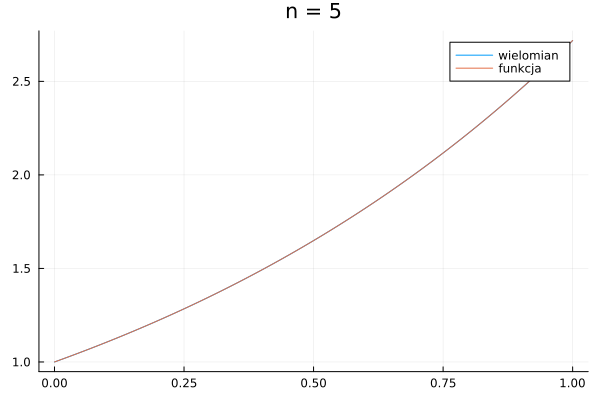
\includegraphics[width=100mm]{z5f1_5.png}
    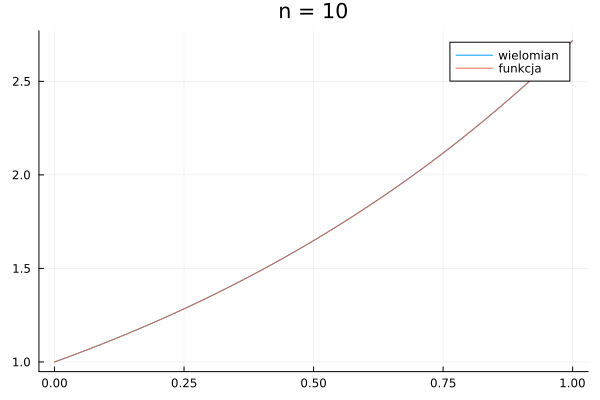
\includegraphics[width=100mm]{z5f1_10.png}
    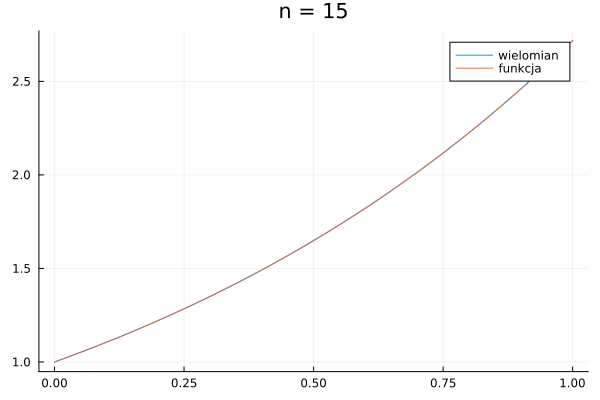
\includegraphics[width=100mm]{z5f1_15.png}
    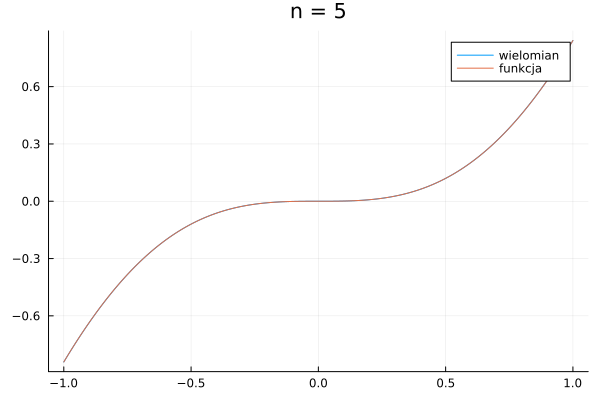
\includegraphics[width=100mm]{z5f2_5.png}
    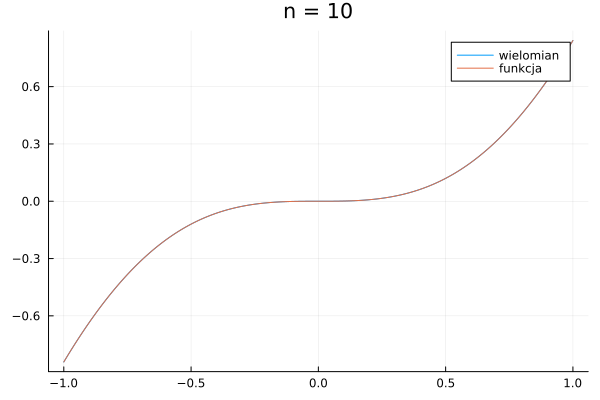
\includegraphics[width=100mm]{z5f2_10.png}
    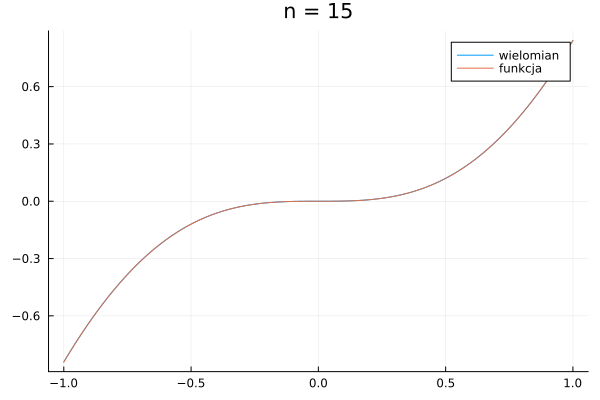
\includegraphics[width=100mm]{z5f2_15.png}
    \subsection{Wnioski}
    \large Przyglądając się powyższym wykresom, możemy z całą pewnością stwierdzić, iż udało się nam bardzo zinterpolować zadane funkcję.
     Wykresy funkcji oraz wielomianu interpolacyjnego niemal się pokrywają, co ciekawe udało się nam to dokonać dla względnie małych stopni tego wielomianu.
     
    \section{Zadanie 6}
    \subsection{Opis problemu}
    \large Zadanie szóste polega na przetestowaniu funkcji \texttt{rysujNnfx(f,a,b,n)} na następujących przykładach: \newline
    \begin{flushleft}
        (a) \(|x|, [-1,1], n = 5,10,15\) \newline
        (b) \(\frac{1}{1+x^2}, [-5, 5], n=5,10,15\) \newline
    \end{flushleft}
    \subsection{Rozwiązanie}
    \large Rozwiązanie zadania szóstego polega, na zaimplementowaniu opowiedniego programu testującego, który wykorzystuje funkcję z zadania 4,
     oraz w którym parametrami zadanymi do funkcji są dane podane przez autora zadania. 
    \subsection{Wyniki}
    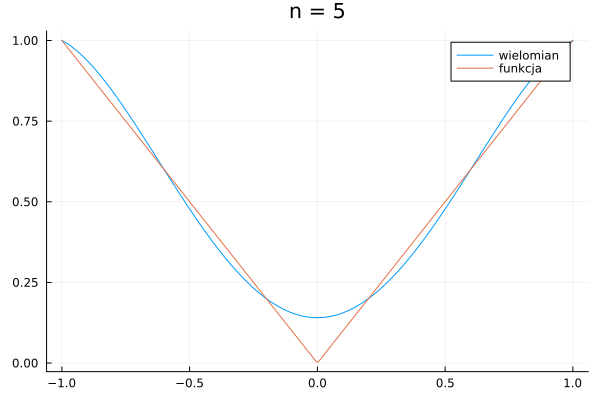
\includegraphics[width=100mm]{z6f1_5.png}
    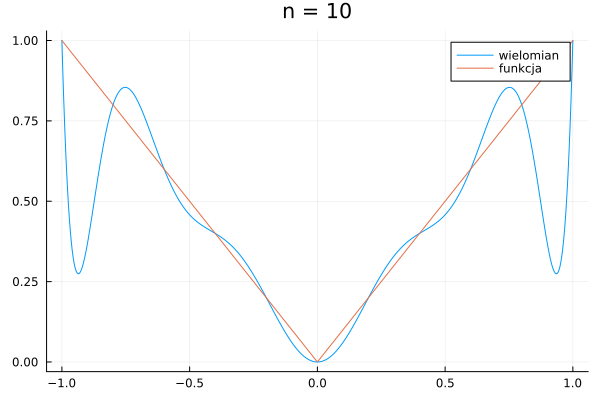
\includegraphics[width=100mm]{z6f1_10.png}
    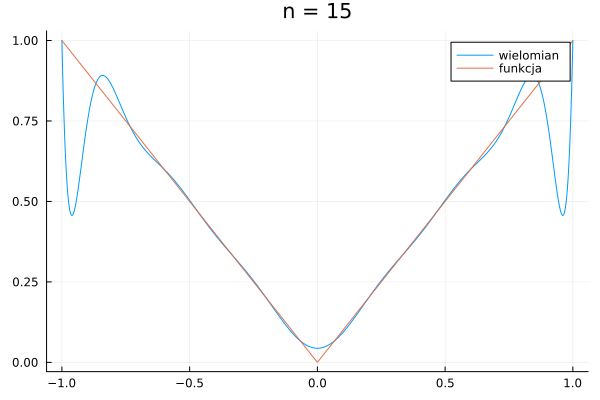
\includegraphics[width=100mm]{z6f1_15.png}
    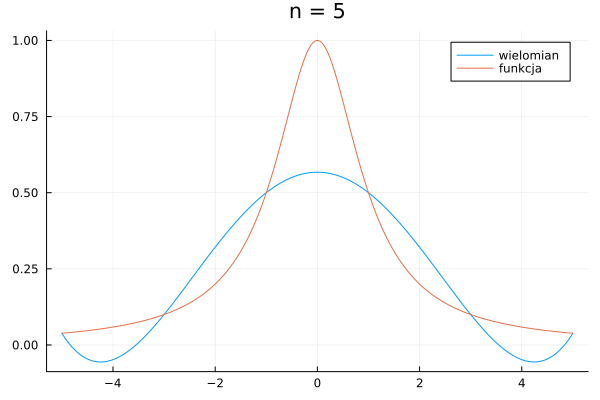
\includegraphics[width=100mm]{z6f2_5.png}
    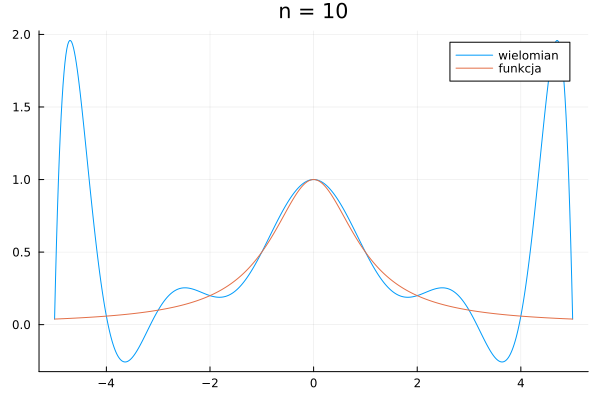
\includegraphics[width=100mm]{z6f2_10.png}
    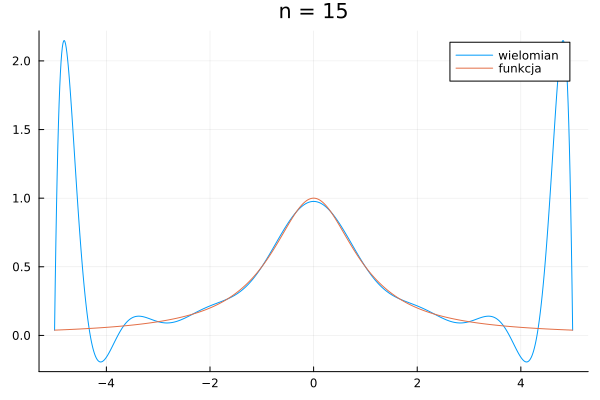
\includegraphics[width=100mm]{z6f2_15.png}

    \subsection{Wnioski}
    Z całą pewnością możemy stwierdzić, że interpolacja wielomianowa jest dobrą metodą przybliżania funkcji, niemniej jednak należy pomiętać o jej ograniczeniach,
    gdyż nie w każdym przypadku możemy otrzymać oczekiwany wynik. W przypadku funkcji z zadania piątego, nasz metoda poradziła sobie wzorowo, lecz w przypadku funkcji takich jak w zadaniu szóstym.
    Zwyczajnie funkcje z zadania szóstego posiadają bardzo ostre kształy, które z pewnością sprawiają bardzo dużo problemów w sytuacji interpolowania.
    Zatem należy się zastanowić, czy ta metoda aby na pewno jest odpowiednia do tego typu funkcji.
    \end{center}
    \begin{thebibliography}{100}
        \bibitem{Kincaid} D. Kincaid, W. Cheney, Analiza numeryczna, Wydawnictwa Naukowo-Techniczne, Warszawa 2006. ISBN 83-204-3078-X
    \end{thebibliography}

\end{document}